\section{Lastenheft}
\label{Lastenheft}
In diesem Kapitel wird auf das Lastenheft eingegangen. Es wird beschrieben wie die Lastfälle bestimmt und definiert wurden.

Damit die Erklärung des Lastenheftes und der gesammte folgende Auslegungsprozess an sich verständlicher wird, werden zuerst die verwendeten Begriffe definiert.\\
Als \emph{Modus} wird ein ``Zustand'' oder eine ``Position'' des Solar Butterflys verstanden. Modus \emph{A} beschreibt zum Beispiel den Solar Butterfly im ``Fahr-Modus''. In diesem Fall würde dies bedeuten, dass alle Panelen, Stützen und Seitenmodule eingefahren sind. Es wird für jeden der vier definierten Modi ein FEM-Modell erstellt.\\
Als \emph{Lastfall} wird eine Situation (z.B. Fahrt auf einer um 10° geneigten Strasse) oder eine Last (z.B. Personenlast) verstanden, welche in einem spezifischen Modus auftreten kann. Der Lastfall \emph{1.1} im Modus \emph{A} beschreibt zum Beispiel die vertikale Beschleunigung von 1.25 g welche durch das Überfahren einer Bresmmschwelle auftreten kann. Der Lastfall \emph{1.1} im Modus \emph{C} beschreibt eine Personenlast. Ein Lastfall ist vollständig definiert, wenn klar ist, wie dieser im jeweiligen FEM-Modell des betreffenden Modus, einzugliedern ist.\\
Der Lastfall \emph{1.1} im Modus \emph{A} ist nicht notwendigerweise der Selbe, wie der Lastfall \emph{1.1} im Modus \emph{B} oder \emph{C}! Die klare Zuweisung der Lastfälle zu einem spezifischen Modus wurde vorgenommen, um die Anzahl der Lastfälle in den verschiedenen Modi gering zu halten und die daraus resultierenden Lastkombinationen pro Modus übersichtlicher zu gestalten. Dies führt mit sich, dass gewisse Lastfälle in mehreren Modi vorkommen und dass dadurch einige Lastfälle doppelt aufgeführt werden. So wird zum Beispiel der Lastfall \emph{Neigung Stehend} im Modus \emph{B} und \emph{C} aufgeführt, da die Situation des geneigten Bodens im parkierten Zustand in beiden Modi auftreten kann. Alle Lastfälle welche in diesen Modi nicht auftreten, können jedoch weggelassen werden, wodurch - wie bereits erwähnt - das Lastenheft übersichtlicher gestaltet werden kann.\\
Zur Beschreibung eines Lastfalles gehört eine Bewertung des dazugehörenden \emph{Risikos}. Ein \emph{Risiko} setzt sich zusammen aus der Ungenauigkeit der Voraussage der Belastung und einer Abschätzung der ``ernsthaftigkeit'' der potentiellen Auswirkungen. Eine \emph{Ungenauigkeit} von 0.5 bedeutet, dass von einer potentiellen Abweichung der Belastung von $\pm\: 50\%$ ausgegangen wird. Für die Werte der \emph{Auswirkungen} wird kein klarer Massstab definiert. Sie nehmen einen Wert zwischen 0 und 100 an und beurteilen die Auswirkungen beim ``Eintreten'' der Ungenauigkeit. Das Produkt aus der Ungenauigkeit und der Auswirkung ergibt den Wert des Risikos.
Ein hoher Risiko-Wert bedeutet nicht, dass die betrefende Last ein grosses Risiko für den Solar Butterfly darstellt, sondern, dass die Abschätzung der Last unsicher ist. Das soeben erkläuterte Risiko ist also ein Mass für die Gefahr, sowie auch für das Potentail, welches in der Abschätzung der Last steckt. Ein Risiko-Wert von 0 bedeutet ausgeschrieben, dass die Last mit grosser Sicherheit so auftreten wird, wie diese im Lastenheft beschrieben ist. Ein hoher Risiko-Wert bedeutet wiederum, dass man sich nicht sicher ist, ob die Last wie beschrieben auftreten wird. Die Last kann zu tief (daher die Gefahr), oder aber auch zu hoch (daher das Potential) gewählt worden sein. Lasten mit hohen Risiko-Werten sollen bei einer Überarbeitung des Lastenheftes erhöhte Beachtung geschenkt werden.\\
Als \emph{Lastkombination} wird eine Kombination von verschiedenen Lastfällen verstanden. Eine Lastkombination bezieht sich jeweils auf einen Modus. Die Lastkombination \emph{A.3.1.2} setzt sich zusammen aus dem Modus \emph{A} und den Lastfällen \emph{1.3 Longitudinale Beschleunigung - Negativ}, \emph{2.1 Wind von links} und \emph{3.2 Neigung längs negativ} aus dem Modus \emph{A}.

Ein Blick in das Lastenheft im Anhang [ANHANG] wird das soeben beschriebene verständlicher machen.\\

\paragraph{Missbrauchslastfälle und Dynamik}
Missbrauchslastfälle: Werden nur für die einzelnen Komponenten berücksichtigt. Weil aufwand sons zu gross?

Die Dynamik der Lastfälle wird in der Grobauslegung nicht ausführlich betrachtet. Der Solar Butterlfy wird jeweils für den Maximalwert - die Amplitude - eines Lastfalles statisch ausgelegt. Die Dynmaik der Lastfälle und die daraus resultierende potentielle Ermüdung der Materialien werden mit entsprechend gewählten Design-Allowables abgedeckt.

Folgend werden die drei Modi mit den dazugehörigen Lastfällen vorgestellt. Es wird jeweils beschrieben, wie die Lasten zustande kommen und wie diese in den FEM-Modellen eingegliedert werden.

\subsection{Modus A: Fahren}
Der Modus \emph{A} beschreibt den Solar Butterfly im ``Fahr-Modus'' und ist in der Abbildung \ref{Modus A} dargestellt. Konkret bedeutet dieser Modus, dass alle Panelen und Seitenmodule eingefahren und über die Verschlüsse fest mit dem Rest des Aufbaus verbunden sind. Ebenfalls sind die alle Stützen eingefahren. Im Fahr-Modus befinden sich keine Personen im Solar Butterfly und das Mobiliar ist an den dafür vorgesehenen Stellen verstaut. Weiter herrscht in allen Lastkombinationen die Erdbeschleunigung von 1 g. Der Lastfall von 1 g wird nicht spezifisch aufgeführt.

\begin{center}
  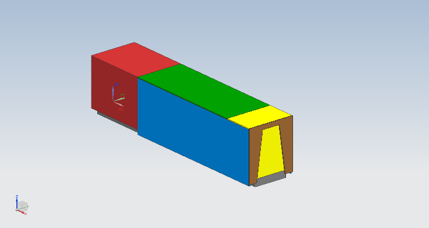
\includegraphics[width=0.5\textwidth]{04_Figures/A.png}
  \captionof{figure}{Modus A}
  \label{Modus A}
\end{center}

  \paragraph{Beschleunigungen durch Fahren}
  \begin{description}
    \item \textbf{1.1 Vertikale Beschleunigung}\\
    Zusätzlich zur vertikalen Beschleunigung durch die Erdanziehung, entstehen durch das Überfahren von Schlaglöcher und Bremsschwellen vertikale Beschleunigungen.\\
    In einem ersten Ansatz die Beschleunigung beim Überfahren einer Bresmmschwelle zu bestimmen, wurde der Solar Butterfly als ein \emph{Ein-Massen-Schwinger}-System modelliert und die Beschleunigung beim Überfahren einer Sinusförmigen Bremsschwelle numerisch ermittelt.\\

    Die Position des Rades während dem Überfahren der Bremsschwelle ist gegeben durch folgenden Zusammenhang:
    \begin{equation}
      x_r^n = h \cdot sin\left(\pi \cdot \frac{n\Delta t \cdot v}{l}\right)
    \end{equation}
    $l$ steht dabei für die Länge, und h für die Höhe der Bremsschwelle.\\

    Um die Beschleunigung des Solar Butterflys zu berechnen, wird in einem ersten Schritt dessen Position zum Zeitpunk $n$ $x_{SB}^n$ aus der vorangehenden Situation berechnet.
    \begin{equation}
      x_{SB}^n = x_{SB}^{(n-1)} + v^{(n-1)} \cdot \Delta t
    \end{equation}

    Als nächstes wird der Federweg $s^n$, sowie die Änderungsrate des Federwegs $v_s^n$ zum Zeitpunkt $n$ aus den Positionen des Rades $r_x^n$ und des Solar Butterflys $x_{SB}^n$ berechnet.
    \begin{equation}
      s^n = x_r^n - x_{SB}^n
    \end{equation}
    \begin{equation}
      v_s^n = \frac{s^n - s^{(n-1)}}{\Delta t}
    \end{equation}

    Die Beschleunigung des Solar Butterfly ergibt sich dann zu:\\
    \begin{equation}
      a_{SB}^n = \frac{k \cdot s^n + d \cdot v_s^n}{m}
    \end{equation}

    Wobei $k$ für die Federkonstante und $d$ für die Dämpfungskonstante stehen.
    Die aus der Beschleunigung des Solar Butterfly resultierende neue Geschwindigkeit, kann wie folgt berechnet werden.
    \begin{equation}
      v^n = v^{(n-1)} + a_{SB}^n \cdot \Delta t
    \end{equation}

    Das \emph{Ein-Massen-Schwinger}-Modell wurde mit einer Masse von 2200 kg, einer mittleren Federkonstante, gegeben aus den Datenblättern des Herstellers [ANHANG], von 353'000 N/m und einer Dämpfungskonstante von 3500 Ns/m modelliert. Beim Überfahren einer Bremsschwelle von 0.9 m Länge und 0.1 m Höhe mit einer Geschwindigkeit von 40 km/h resultiert eine maximale Beschleunigung von rund 1.6 g. Die Berechnung ist im elektronischen Anhang [Elektronischen Anhang] einsehbar.\\
    Zu der Berechnung muss gesagt werden, dass davon ausgegangen werden kann, dass die erhaltene Beschleunigung zu hoch liegt. So wurde zum Beispiel die Federung durch die Reifen nicht berücksichtigt. Weiter befindet sich der Massenschwerpunkt nicht in der Federachse, was eine weitere Abminderung der Beschleunigung zur folge hat.\\

    Um die zu wählende Beschleunigung breiter abstützen zu können, wurden andere Arbeiten zum Thema herbeigezogen. \emph{Janczur} \cite{Beschl.1} zeigt, dass beim Überfahrein einer Bremsschwelle von 0.36 m Länge und einer Höhe von 0.05 m, mit einer Geschwindigkeit von 40 km/h, in der Fahrzeugmitte eines Personenwagens, Beschleunigungen von 0.71 g herrschen. Direkt über der Fahrzeugachse treten Beschleunigungen von bis zu 1.5 g auf.\\
    \emph{García-Pozuelo} et al. \cite{Beschl.2} massen in der Fahrzeugmitte eines Personenwagens Beschleunigungen von 0.73 g beim Überfahrein einer Bremsschwelle von 0.9 m Länge und 0.1 m Höhe. Dies bei einer Geschwindigkeit von 50 km/h.\\
    \emph{Haniszewski} et al. \cite{Beschl.3} massen Beschleunigungen, welche eine Person auf der Rückfahrbank eines Personenwagens während dem Überfahren einer Bremsschwelle erfährt. Sie massen Beschleunigungen von bis zu 1 g. Direkt über der Fahrzeugachse wurden Beschleunigungen von 1.3 g gemessen. Dies bei einer Geschwindigkeit von 30 km/h und einer Bremsschwelle von 0.5 m Länge und 0.05 m Höhe.\\
    \emph{Pidl} \cite{Beschl.4} zeigt, dass Transportware in einem Sattelschlepper Beschleunigungen von $\pm$ 1 g erfahren. Ob diese maximal gemessene Beschleunigung beim Überfahren einer Bremsschwelle erreicht wurde, ist nicht ersichtlich.

    Da der Achsenabstand des Solar Butterflys, im vergleich zu den Personenwagen aus der Literatur, relativ klein ist, werden die in der Fahrzeugmitte gemessenen Beschleunigungen der Personenwagen nicht als räpresentative Näherungswerte für die Beschleunigung des Solar Butterflys verwendet. Es wird davon ausgegangen, dass die Beschleunigungen, welcher ein Personenwagen dirket über der Achse beim Überfahren einer Bremsschwelle erfäht, vergleichbar mit jenen sind, welche der Solar Butterfly erfahren wird. Diese Annahme wird getroffen, da die Achsen des Solar Butterflys nahe beisammen liegen und eher den letzteren Fall beschreiben.\\
    Aufgrund den getroffenen Annahemn wird die Beschleunigung von 1.5 g als erste Abschätzung festgelegt. Hinsichtlich den grossen Unsicherheit der Annahmen wird die \emph{Ungenauigkeit} auf 0.4 geschätzt. Die \emph{Auswirkung} werden dabei mit einem Wert von 50 festgelegt was einen hohen Risikowert von 20 ergibt.

    \item \textbf{1.2 Longitudinale Beschleunigung - Positiv (Erhöhen der Geschwindigkeit)}\\
    Longitudinale positive Beschleunigungen in Fahrtrichtung entstehen durch eine Erhöhung der Fahrgeschwindigkeit durch das Zugfahrzeug. Das \emph{Institut für Unfallanalysen Hamburg} \cite{Verz.3} benützt die Beschleunigung von Personenwagen von maximal 0.3 g und von Lastkraftwagen von 0.1 g, als Anhaltswerte.

    Für das Lastenheft wird die Beschleunigung von 0.2 g gewählt. Sie wird höher als der Anhaltswert des Institut für Unfallanalysen Hamburg für Lastkraftwagen von 0.1 g gewählt, da das geplante Zugfahrzeug ein elektrisches ist, und dadurch höhere mögliche Beschleunigungen erwartet werden können. Die \emph{Ungenauigkeit} wird mit 0.2 als gering eingestuft. Ebenfalls wird die \emph{Auswirkung} von 20 als niedrig bewertet.

    \item \textbf{1.3 Longitudinale Beschleunigung - Negativ (Bremsen)}\\
    Longitudinale Verögerungen entstehen durch abminderung der Fahrgeschwindigkeit. Die extremste graduelle Verzögerung entsteht dabei durch eine Notbremsung.\\
    \emph{Kudarauskas} \cite{Verz.1} zeigt bei seiner Analyse der Notbremsungen von Personenwagen, dass die maximalen Verzögerungn bei rund 0.9 g liegen. Das \emph{Institut für Unfallanalysen Hamburg} \cite{Verz.2} zeiht bei Gutachten die Vollverzögerung von 0.8 g für Personenwagen und 0.7 g für Lastkraftwagen als Standardwerte herbei.

    Für die longitudinale Beschleunigung durch Bremsungen wird sich am Institut für Unfallanalysen Hamburg orientiert und ein Wert von 0.7 g gewählt. Dies, da davon ausgegangen wird, dass die maximalen Verzögerungen von \emph{Kudarauskas} von 0.9 g mit dem Solar Butterfly nicht erreicht werden können. Weiter wird angenommen, dass das Verhalten eines Lastkraftwagens während einer Vollverzögerung die Situation des Solar Butterflys ähnlicher beschreibt als jenes des Personenwagens.
    Die longitudinale Beschleunigung wird mit einer \emph{Ungenauigkeit} von 0.2 und einer \emph{Auswirkung} von 30 bewertet.

    \item \textbf{1.4 Laterale Beschleunigung}\\
    Laterale Beschleunigungen entstehen vorallem beim Kurvenfahren und sind abhängig von der Geschwindigkeit mit welcher die Kurve durchfahren wird und des Kurvenradius.\\
    \emph{Hugemann} et al. \cite{Kurv.1} massen in einem Personenwagen auf einer Landstrasse laterale Beschleunigungen von 0.6 g. \emph{Xu} et al. \cite{Kurv.2} zeigten, dass die Mehrheit der gemessenen Beschleunigung in einem Personenwagen durch Kurvenfahrten in bergigem Gebiet über 0.5 g und maximale über 0.8 g liegen.

    Da davon ausgegangen wird, dass mit dem Solar Butterfly die Kurven vorsichtiger, und somit tendenziell langsamer durchfahren werden als mit einem Personenwagen, wird die laterale Beschleunigung von 0.8 g als ein passenden Anhaltswert erachtet. Es wird erwatet, dass die nach \emph{Xu} et al. höher als 0.8 g liegende Beschleunigungen nicht erreicht werden. Die \emph{Ungenauigkeit} wird mit 0.1 als gering bewertet. Die \emph{Auswirkung} wird auf 70 geschätzt.

    \item \textbf{1.5 Rotatorische Beschleunigung}\\
    Rotatorische Beschleunigungen können durch eine in querrichtung unebene Strassen verursacht werden. Beim Überfahren einer solchen Strasse neigt sich der Solar Butterfly abwechslungsweise nach links und rechts, wodurch rotatorische Beschleunigungen auftreten. Um diese Beschleunigungen abschätzen zu können wird die folgende Berechnung durchgeführt:

    Die folgende Gleichung beschreibt den Neigungswinkel $\varphi$ des Solar Butterflys in abhängigkeit der Zeit $t$:
    \begin{equation}
      \varphi(t) =  \varphi \cdot \sin \left(\omega t \right)
    \end{equation}

    wobei $\varphi$ für die maximale Neigung steht und $\omega$ sich wie folgt berechnen lässt:
    \begin{equation}
      \omega = \frac{2\cdot \pi}{T}
    \end{equation}
    Wobei $T$ für die Dauer einer Schwingung (Neigung von rechts nach links und wieder zurück) steht.\\
    Die Winkelbeschleunigung $\alpha$ ergibt sich aus der zweiten Ableitung von $\varphi(t)$ und lässt sich wie folgt berechnen:
    \begin{equation}
      \alpha(t) = \ddot \varphi(t) = -\Delta\varphi\:\omega^2 \cdot \sin \left(\omega t \right)
    \end{equation}

    Mit einer Schwingdauer von einer Sekunde und einer maximalen Neigung $\varphi$ von 6.5°, welche sich aus einem Höhenunterschied des Rades von 200 mm und dem Radstand des Solar Butterflys von 1770 mm ergibt, resultiert eine maximale Winkelbeschleunigung von $4.4 \; \frac{rad}{s^2}$.\\
    Da die realen Bedingungen einer solchen Situation nur schwer abgeschätzt werden können, wird die \emph{Ungenauigkeit} mit 0.3 hoch angesetzt. Ebenfalls können die Auswirkungen einer solchen Beschleunigung nur schwer beurteilt werden, weshalb die \emph{Auswirkung} auf 60 gesetzt wird.
  \end{description}

  \paragraph{Windlasten}\mbox{}\\
  \emph{Sesar} et. al \cite{Wind.1} zeigen, dass laterale Windgeschwindigkeiten von 108 $\frac{km}{h}$ für Fahrzeuge auf trockener Strasse kritische seien.\\
  Die Blog-Seite \emph{rvblogger.com} \cite{Wind.2} empfiehlt bei Windgeschwindigkeiten von mehr als 80 $\frac{km}{h}$ mit einem Wohnwagen nicht mehr zu Fahren. Windgeschwindigkeiten von 95 $\frac{km}{h}$ seien laut \emph{rvblogger.com} genug, um Wohnmobile umzustossen.\\
  Bei Windgeschwindigkeiten von mehr als 155 km/h können laut \emph{Beasley} \cite{Wind.3} Lastwagen mit hohem Profil, Anhänger und Busse umkippen. Die berichteten minimale Überschlagswindgeschwindigkeiten sind 105 $\frac{km}{h}$ für ein 9 Meter langen Wohnwagen und 160 $\frac{km}{h}$ für ein 5 Meter langes Wohnmobil (Klasse B).

  Für eine erste Abschätzung der zugelassenen Windgeschwindigkeit bei der Fahrt des Solar Butterfly wird sich an der Blog-Seite \emph{rvblogger.com} orientiert und die Geschwindigkeit von 80 $\frac{km}{h}$ als Limitte festgelegt. Für die Berechnung der durch den Wind entstehenden Belastung, wird der Solar Butterfly vereinfacht als noraml angeströmtes Rechteck betrachtet. Für die Berechnung des Winddruckes wird die erhöhte Geschwindigkeit von 102.2 $\frac{km}{h}$ (Beaufort 10) verwendet um Böhen und eventuelle Ungenauigkeiten in der Messung oder Abschätzung der Windgeschwindigkeiten abzudecken. Der Winddruck wird gemäss Formel \ref{Winddruck} berechnet.

  \begin{equation}
    \label{Winddruck}
    P_W = c_p \: \frac{\rho}{2}\: v^2
  \end{equation}

  Wobei für die Dichte von Luft $\rho$ ein Wert von $1.2 \frac{kg}{m^3}$ und für den Strömungswiderstandskoeffizient eines Rechteckes $c_{p,Rechteck}$ ein Wert von $1.1$ gewählt wird. Bei einer Windgeschwindigkeit von 102.2 $\frac{km}{h}$ ergibt sich gemässt der Gleichung \ref{Winddruck} ein Winddruck von $532 \; Pa$.

  Da es sich hierbei um eine grobe Idealsierung handelt und zum Beispiel lokale Geschwindigkeitserhöhungen oder Turbulenzen vernachlässigt werden, wird die \emph{Ungenauigkeit} auf 0.4 gesetzt. Die \emph{Auswirkung} wird jedoch eher tief, mit dem Wert 10 bewertet.

  \begin{description}
    \item \textbf{2.1 Wind von links}\\ Der Winddruck von $532  \; Pa$ wirkt auf die, in Fahrtrichtung gesehen, linke Seite des Solar Butterfly.
    \item \textbf{2.2 Wind von rechts}\\ Der Winddruck von $532 \; Pa$ wirkt auf die, in Fahrtrichtung gesehen, rechte Seite des Solar Butterfly.
  \end{description}

  \paragraph{Neigung}\mbox{}\\
  Mittels einer Absprache mit \emph{Palmer} wurde eine zulässige Strassenneigung für den Solar Butterfly von 10° (17.5\%) definiert. Die Strasse auf den Furkapass hat zum Vergleich eine maximale Neigung von 6.3° (11\%). Die verschiedenen Lastfälle der Neigung treten nicht gleichzeigtig ein. Implementiert werden die Fälle im FEM indem die Richtung, in welcher die Erdbeschleunigung wirkt, verändert wird. Die \emph{Ungenauigkeit} und die \emph{Auswirkung} werden tief mit den Werten 0.1  und 10 bewertet.

  \begin{description}
    \item \textbf{3.1 Neigung längs positiv} +10° Neigung des Untergrundes in Fahrtrichtung.
    \item \textbf{3.2 Neigung längs negativ} -10° Neigung des Untergrundes in Fahrtrichtung.
    \item \textbf{3.3 Neigung quer positiv} +10° Neigung des Untergrundes noraml zur Fahrtrichtung. Ansteig befindet sich in Fahrtrichtung rechts.
    \item \textbf{3.4 Neigung quer negativ} -10° Neigung des Untergrundes noraml zur Fahrtrichtung. Ansteig befindet sich in Fahrtrichtung links.
  \end{description}

  % \paragraph{Mobiliar}\mbox{}\\
  % Gemäss der Anforderungsliste werden sich bis zu 50 kg Mobiliar im Solar Butterfly befinden. Während der Fahrt (Modus A) befindet sich das Mobiliar an der Seitenwand im inneren Seitenmodul.
  %
  % \emph{Ungenauigkeit} 0.4, da grosse ungewissheit bei der Befestigung des Mobiliars. Art der Einleitung ist unbekannt.
  % \emph{Auswirkung} 20, ebenfalls nicht zu vernachlässigen da je nach Art der Befestigung die Konstruktion angepasst werden muss.
  % \begin{description}
  %   \item \textbf{4.1 Mobiliar}\\
  %   !!!!! Wie wird das im FEM gemacht? !!!!!
  % \end{description}

  %=============================================================================
  %                                 Modus B
  %=============================================================================
\subsection{Modus B: Ausfahren}
Die Modi \emph{B1}, \emph{B2} und \emph{B3} beschreiben den Solar Butterfly während dem Ausfahrvorgang der Seitenmodule. Im Modus \emph{B1} sind die Stützen am Chassis unten, alle Seitenmodule und Panelen sind Eingefahren. Dieser Modus stellt den Solar Butterfly im ``Parkierten'' Zustand dar. Bei extremen Umwelteinflüssen wie Schneefall oder starkem Wind, stellt der Modus \emph{B1} den geschütztesten Zustand dar und muss somit diesen extremen Umwelteinflüssen stand halten können.
Im Modus \emph{B2} ist, zusätzlich zu den Stützen am Chassis, das grosse Seitenmodul (In der Abbildung \ref{Modus B2} orange dargestellt) ausgefahren. Standardmässig werden beide Seitenmodule zur selben Zeit ausgefahren. Sollte dies aufgrund von technischen Problemen nicht möglich sein und die Seitenmodule müssen ``von Hand'' einzeln ein- oder ausgefahren werden, wird der Modus \emph{B2} eingenommen. Im Modus \emph{B3} sind beide Seitenmodule ausgefahren.
Auch in diesen drei Modi herrscht die Erdbeschleunigung von 1 g, welche wiederum nicht als Lastfall aufgeführt wird. Während dem Ausfahrvorgang befinden sich keine Personen im Fahrzeug und das Mobiliar befindet sich an der dafür vorgesehenen stellen, wie dies im Modus \emph{A} zuvor bereits der fall war.

\begin{figure}[!ht]
  \centering
    \begin{subfigure}{.333\textwidth}
      \centering
      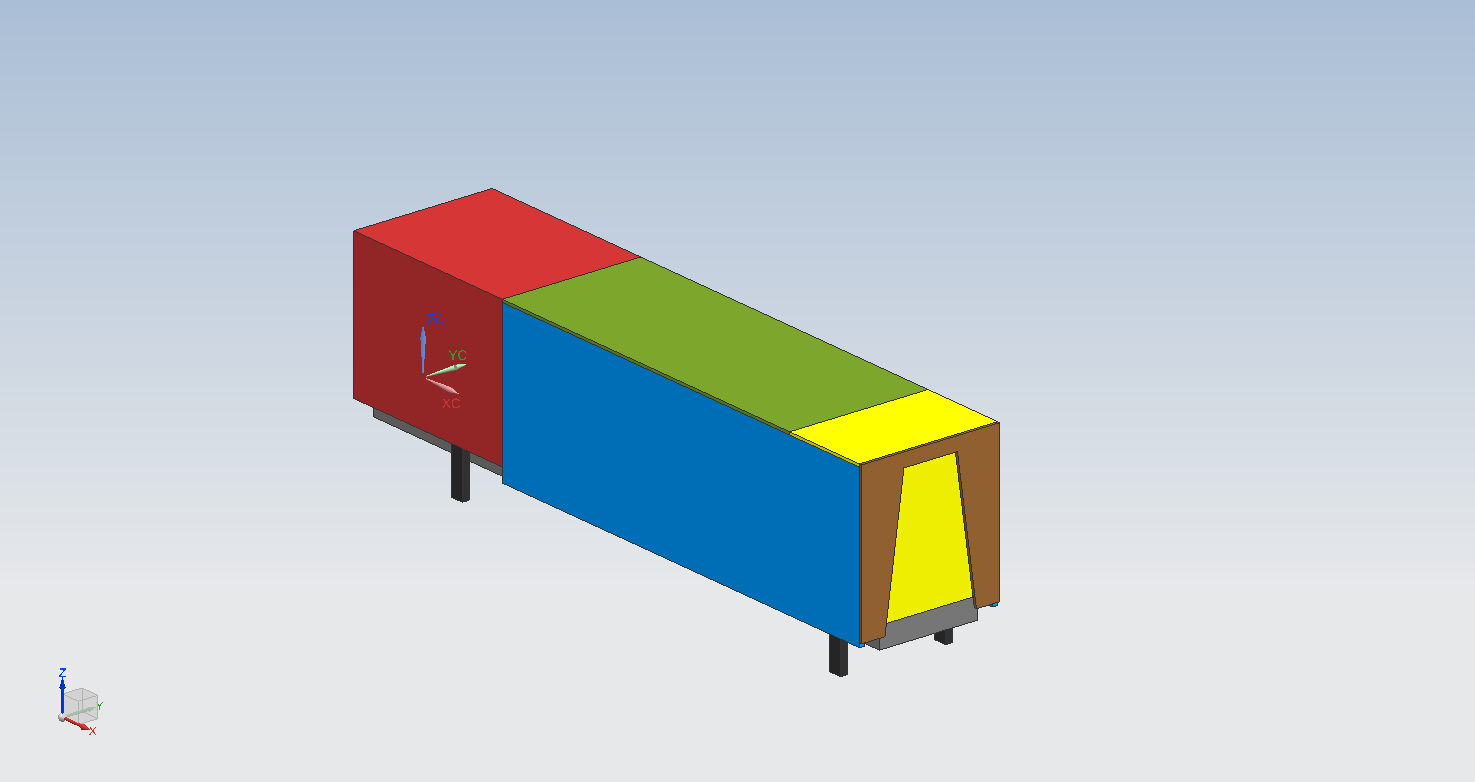
\includegraphics[width=.98\linewidth]{04_figures/B1.png}
      \caption{Modus B1}
      \label{Modus B1}
    \end{subfigure}%
    \begin{subfigure}{.333\textwidth}
      \centering
      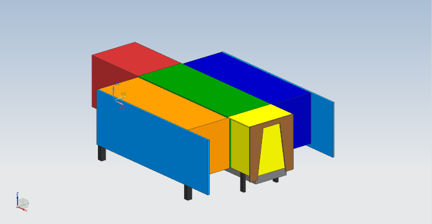
\includegraphics[width=.98\linewidth]{04_figures/B2.png}
      \caption{Modus B2}
      \label{Modus B2}
    \end{subfigure}%
    \begin{subfigure}{.333\textwidth}
      \centering
      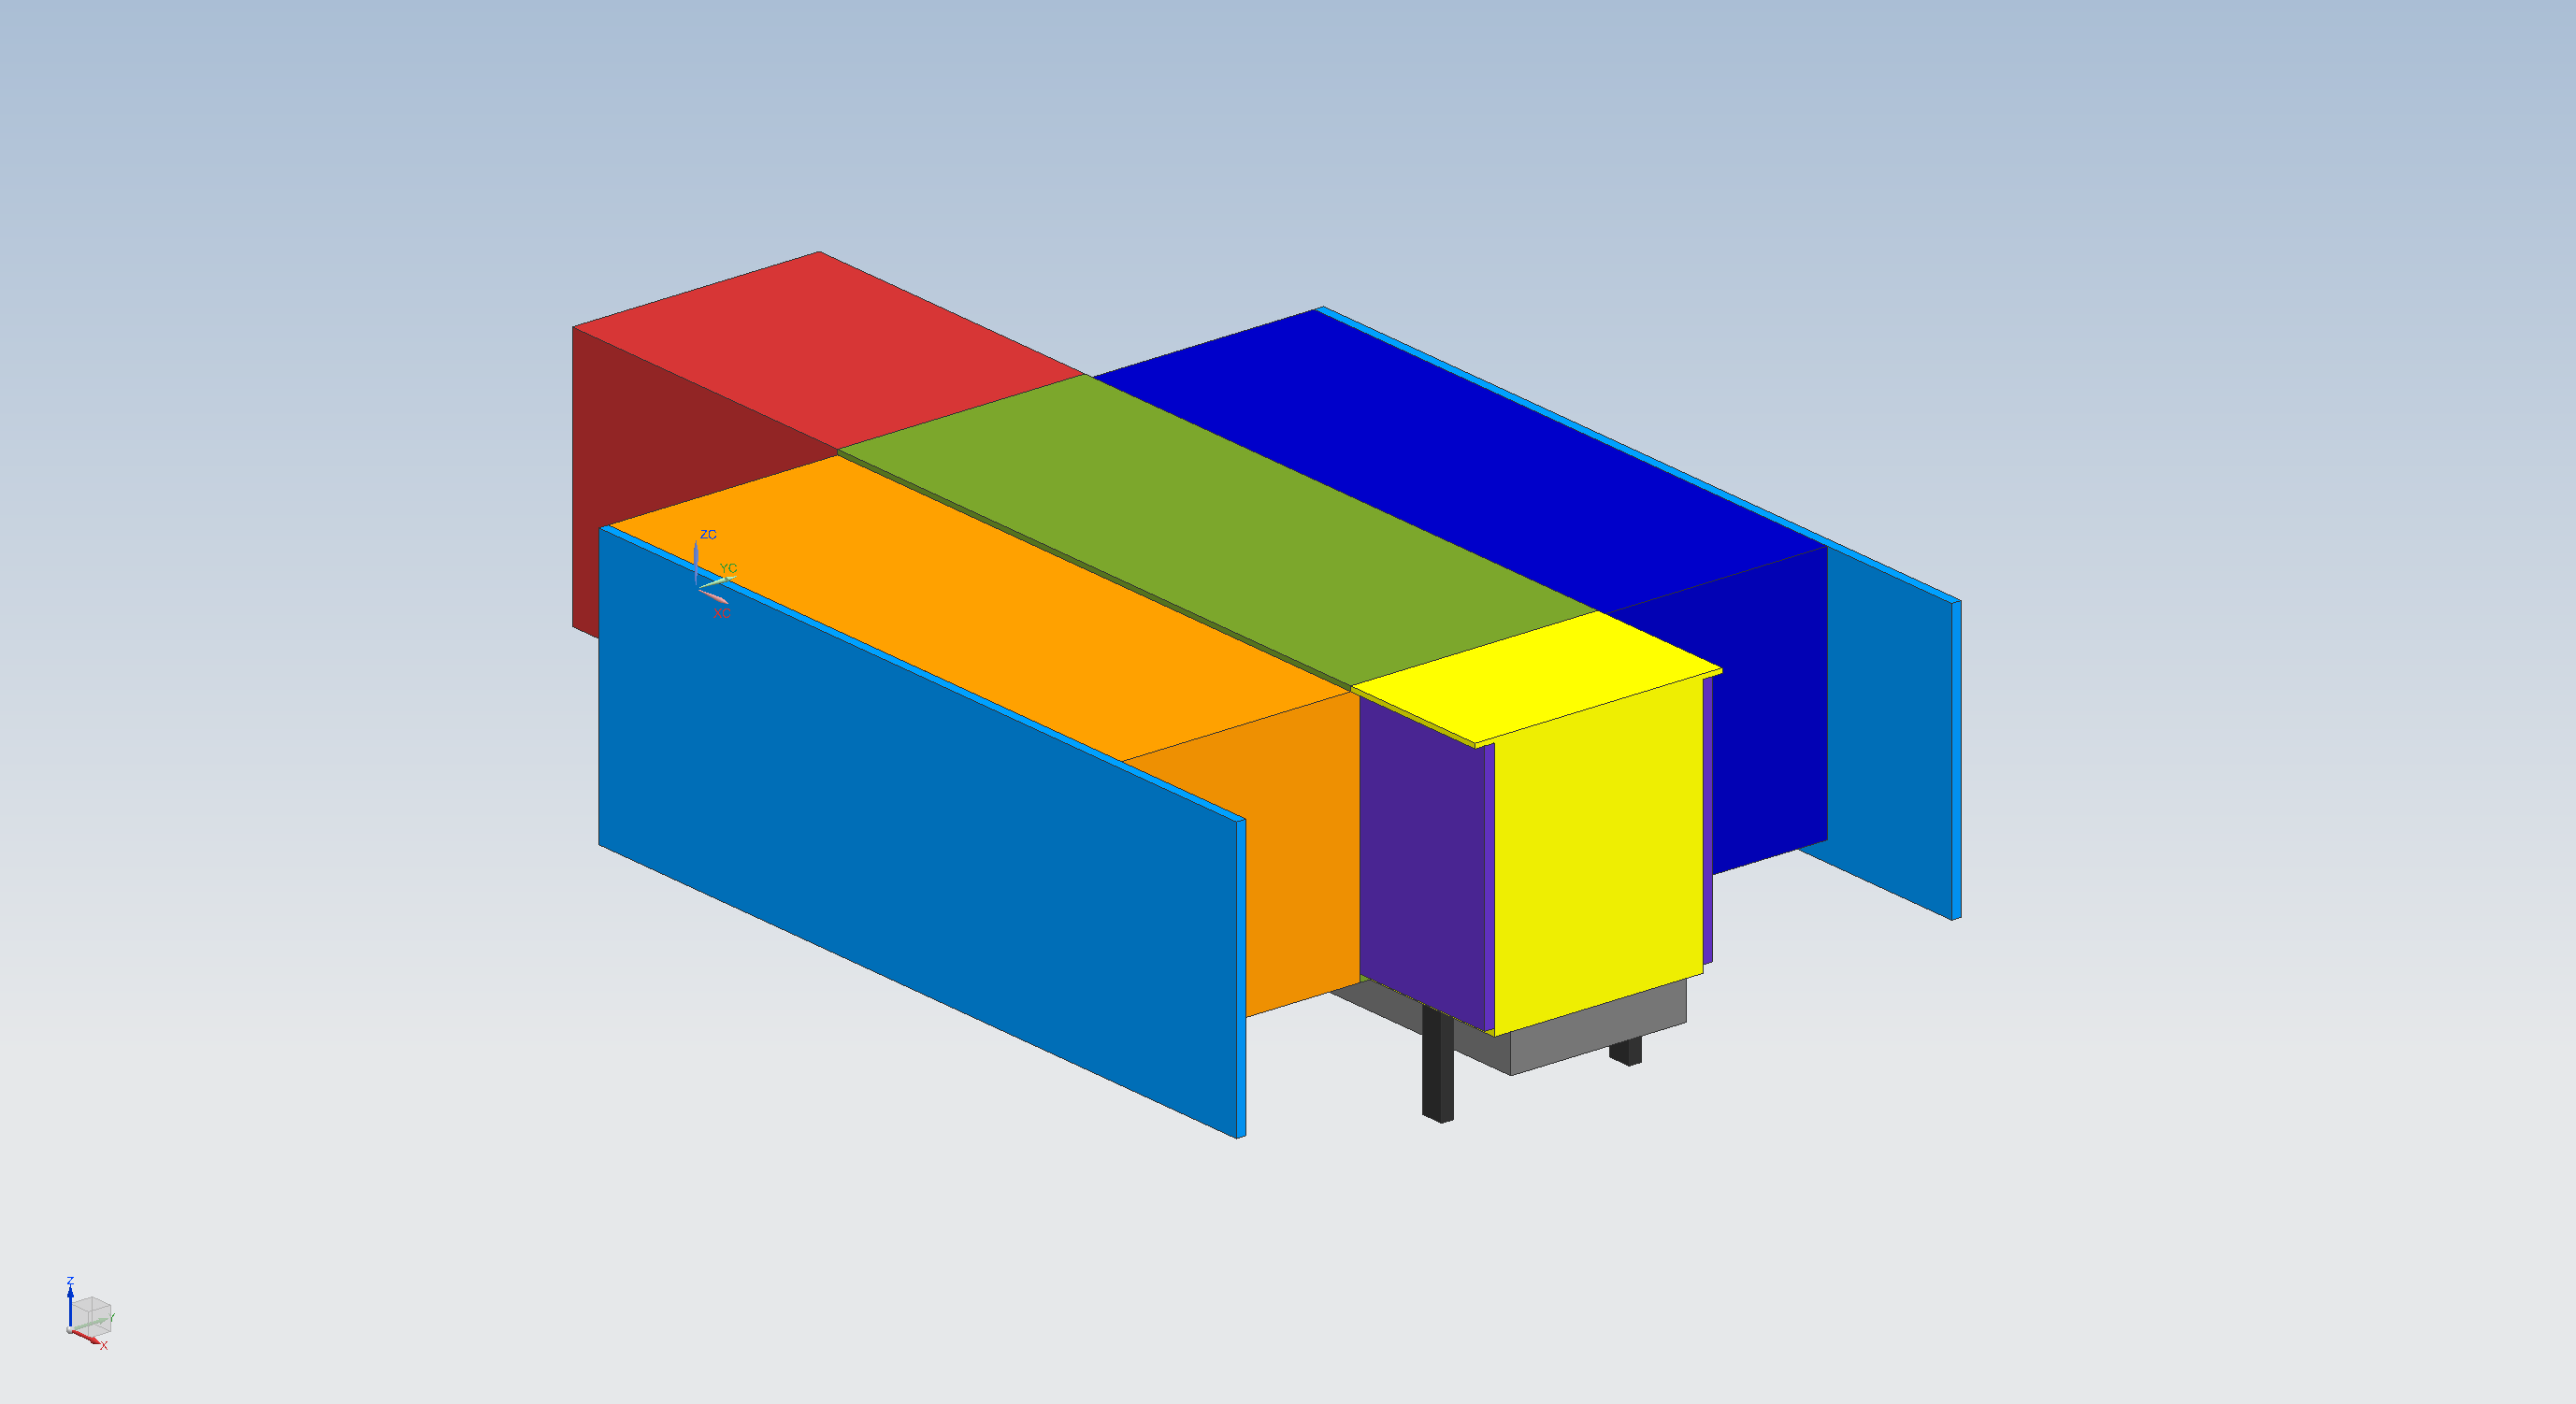
\includegraphics[width=.98\linewidth]{04_figures/B3.png}
      \caption{Modus B3}
      \label{Modus B3}
    \end{subfigure}
  \caption{Modi beim Ausfahren}
\label{Modi beim Ausfahren}
\end{figure}

\paragraph{Windlasten}\mbox{}\\
Windlast von Panelen übernommen
\begin{description}
  \item \textbf{1.1 Wind extrem links}\\
  \item \textbf{1.2 Wind extrem rechts}\\
  Winddruck bei 120 km/h (Orkan, Beaufort 12)?\\
  Eher unsicher, kann viel höher liegen. daher nur erste annahme\\
  Ungenauigkeit 0.4, Auswirkungen 40
  \item \textbf{1.3 Wind von links}\\ Der Winddruck von $486 \; Pa$ wirkt auf die, in Fahrtrichtung gesehen, linke Seite des Solar Butterfly.
  \item \textbf{1.4 Wind von rechts}\\ Der Winddruck von $486 \; Pa$ wirkt auf die, in Fahrtrichtung gesehen, rechte Seite des Solar Butterfly.
  Winddruck bei 120 km/h (Orkan, Beaufort 10)?\\
  Eher unsicher, kann viel höher liegen. daher nur erste annahme\\
  Ungenauigkeit 0.4, Auswirkungen 20
\end{description}

\paragraph{Neigung}\mbox{}\\
Mit Palmer wurde abgesprochen, dass der Boden, auf welchem der Solar Butterfly parkiert wird, die Neigung von 5° (8.8\%) nicht überschreiten darf. Die Implementierung dieser Fälle wird analog zu den Neigungsfällen 3.1 bis 3.4 im Modus \emph{A} durchgeführt. Das Risiko wird ebenfalls analog zu den Neigungsfällen im Modus \emph{A} bewertet.
\begin{description}
  \item \textbf{2.1 Neigung längs positiv} +5° Neigung des Untergrundes in Fahrtrichtung.
  \item \textbf{2.2 Neigung längs negativ} -5° Neigung des Untergrundes in Fahrtrichtung.
  \item \textbf{2.3 Neigung quer positiv} +5° Neigung des Untergrundes noraml zur Fahrtrichtung. Ansteig befindet sich in Fahrtrichtung rechts.
  \item \textbf{2.4 Neigung quer negativ} -5° Neigung des Untergrundes noraml zur Fahrtrichtung. Ansteig befindet sich in Fahrtrichtung links.
\end{description}

% \paragraph{Mobiliar}\mbox{}\\
% Der Lastfall des Mobiliars wird analog zum Lastfall \emph{4.1 Mobiliar} im Modus \emph{A} implementiert und wird hier nur der Vollständigkeit halber aufgeführt.
% \begin{description}
%   \item \textbf{3.1 Mobiliar}\mbox{}\\
%   Bla Bla. Text von oben kopieren.
% \end{description}

%=============================================================================
%                                 Modus C
%=============================================================================
\subsection{Modus C: Ausgefahren}
Der Modus \emph{C} beschreibt den Solar Buttefly im ausgefahren Zustand. Alle Panelen, Stützen und Seitenmodule sind ausgefahren. Personen und das Mobiliar können frei im Solar Butterfly verteilt sein.\\

\begin{center}
  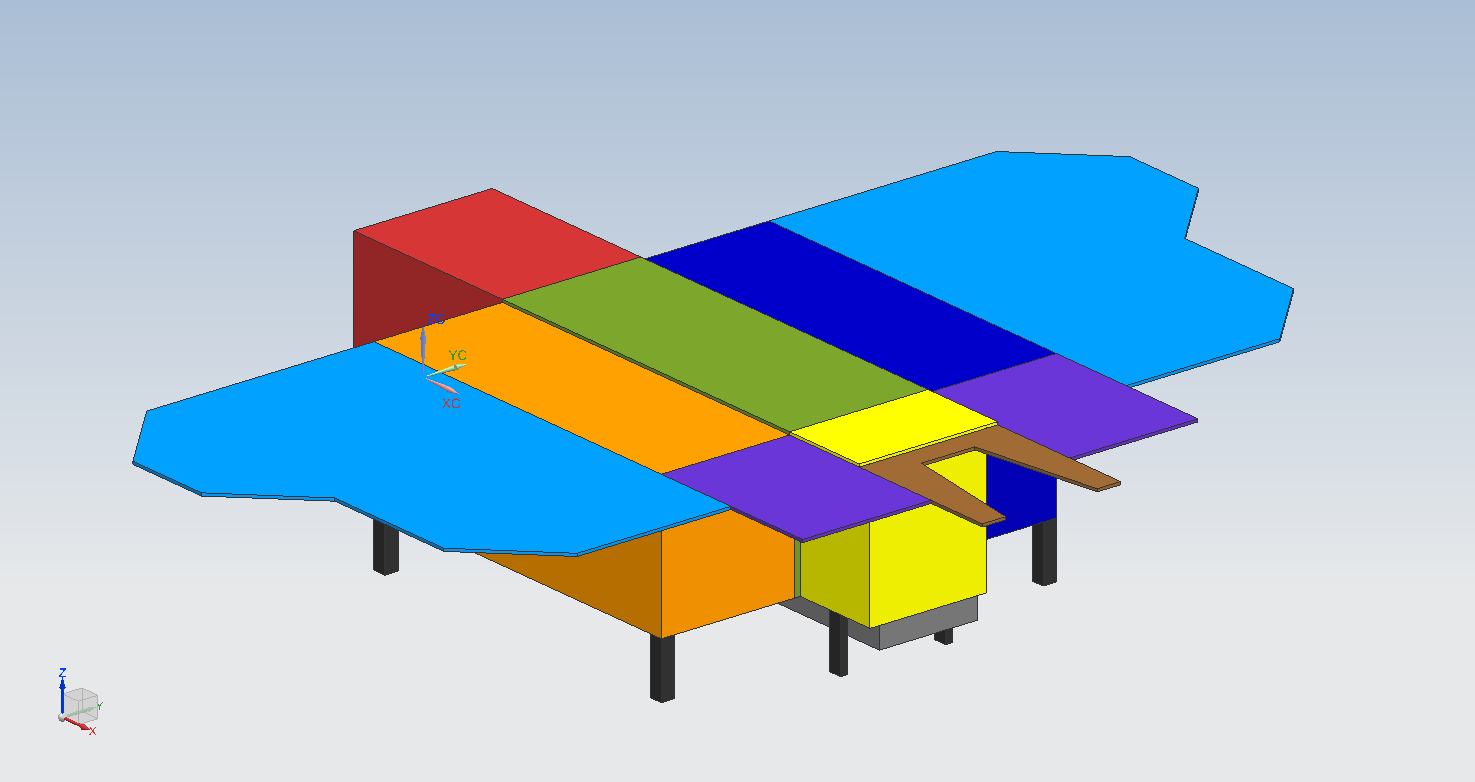
\includegraphics[width=0.5\textwidth]{04_Figures/C.png}
  \captionof{figure}{Modus C}
  \label{Modus C}
\end{center}

\paragraph{Personenlast}\mbox{}\\
Als \emph{Personenlast} werden Lasten verstanden, welche durch Personen, welche sich im inneren des Solar Butteflys befinden, verursacht werden. Aus der Anforderungsliste ist zu entnehmen, dass sich bis zu sechs Personen im Solar Butterfly befinden können sollen. Im Kopf, sowie im Heck des Solar Butterfly, hat es jedoch platzbedingt nur Raum für maximal drei Personen. Das durchschnittliche Gewicht einer Person wird auf 80 kg geschätzt. Die Lastfälle \emph{1.1} bis \emph{1.6} werden als Vektorlasten, die Fälle \emph{1.7} und \emph{1.8} als Flächenlasten im FEM-Modell eingeleitet.

\begin{center}
  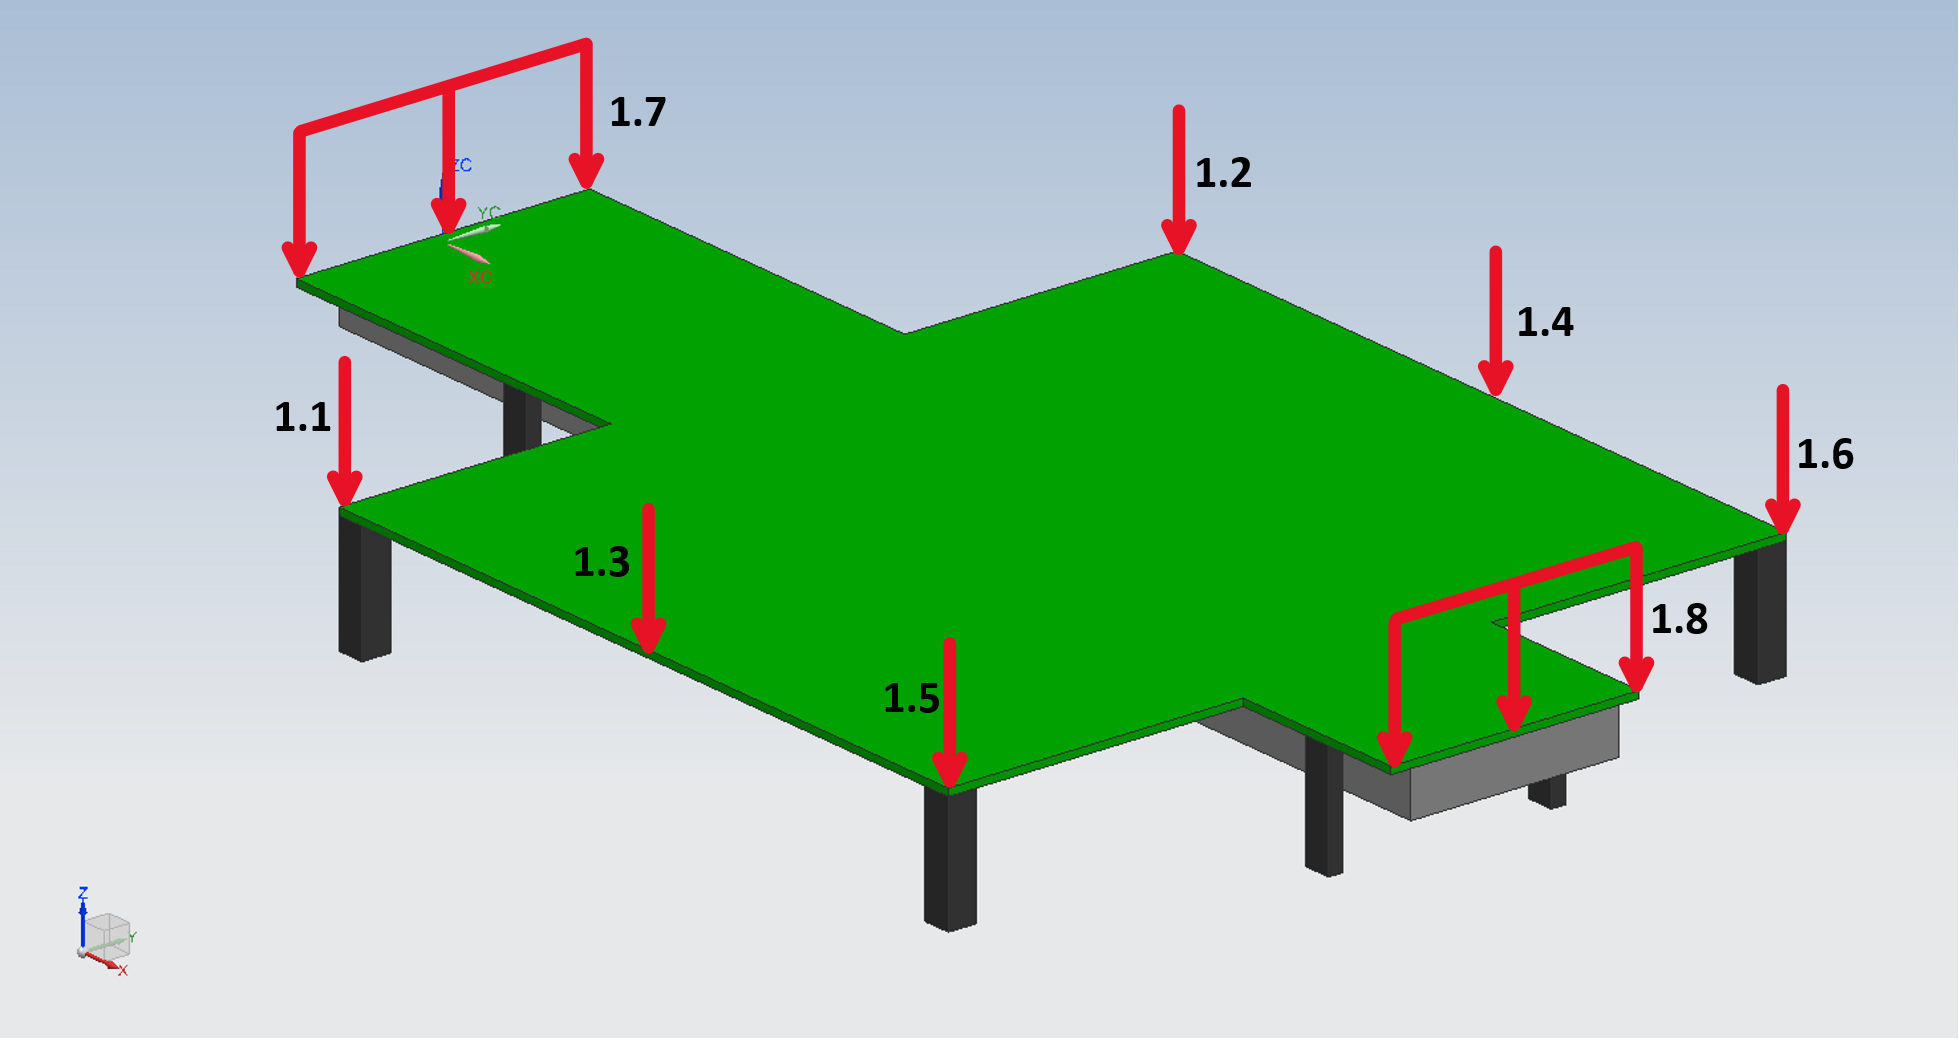
\includegraphics[width=0.8\textwidth]{04_Figures/BodenMitLasten.png}
  \captionof{figure}{Visualisierung der Personenlasten}
  \label{Boden}
\end{center}

\begin{description}
  \item \textbf{1.1 Personenlast vorne links}\\
  6 Personen à 80 kg befinden sich in der vorderen linken Ecke des linken Seitenteils.
  \item \textbf{1.2 Personenlast vorne rechts}\\
  6 Personen à 80 kg befinden sich in der vorderen rechten Ecke des rechten Seitenteils.
  \item \textbf{1.3 Personenlast mitte links}\\
  6 Personen à 80 kg befinden sich in der Mitte der äusseren Kante des linken Seitenteils.
  \item \textbf{1.4 Personenlast mitte rechts}\\
  6 Personen à 80 kg befinden sich in der Mitte der äusseren Kante des rechten Seitenteils.
  \item \textbf{1.5 Personenlast hinten links}\\
  6 Personen à 80 kg befinden sich in der hinteren linken Ecke des linken Seitenteils.
  \item \textbf{1.6 Personenlast hinten rechts}\\
  6 Personen à 80 kg befinden sich in der hinteren rechten Ecke des rechten Seitenteils.
  \item \textbf{1.7 Personenlast Kopf}\\
  Die aus dem Gewicht von 3 Personen à 80 kg resultierende Kraft wird als Flächenlast auf den Boden im Kopf eingeleitet.
  \item \textbf{1.8 Personenlast Heck}\\
  Die aus dem Gewicht von 3 Personen à 80 kg resultierende Kraft wird als Flächenlast auf den Boden im Heck eingeleitet.
\end{description}

Der Fall, dass Personen in der Mitte eines Seitenteils stehen wird im Lastenheft nicht aufgeführt, da davon ausgegangen wird, dass dieser Fall für die globalen Kraftverläufe kein Extrem darstellt. Dieser Fall wird jedoch spezifisch in der Auslegung der Bodenplatten im Kapitel [KAPITEL] berücksichtigt.

\paragraph{Neigung}\mbox{}\\
Die Lastfälle der Neigung sind analog zum den Lastfällen der Neigung im Modus \emph{B}.
\begin{description}
  \item \textbf{2.1 Neigung längs positiv}\\
  +5° Neigung des Untergrundes in Fahrtrichtung.
  \item \textbf{2.2 Neigung längs negativ}\\
  -5° Neigung des Untergrundes in Fahrtrichtung.
  \item \textbf{2.3 Neigung quer positiv}\\
  +5° Neigung des Untergrundes noraml zur Fahrtrichtung. Ansteig befindet sich in Fahrtrichtung rechts.
  \item \textbf{2.4 Neigung quer negativ}\\
  -5° Neigung des Untergrundes noraml zur Fahrtrichtung. Ansteig befindet sich in Fahrtrichtung links.
\end{description}

\paragraph{Mobiliar}\mbox{}\\
Die Belastungen durch das Mobiliar werden jeweils als Flächenlast im FEM-Modell eingeleitet. Die \emph{Ungenauigkeit} sowie die \emph{Auswirkungen} der folgenden Lastfälle wird mit den Werten 0.1 und 10 als gering eingeschätzt.
\begin{description}
  \item \textbf{3.1 Mobiliar Hauptmodul}\\
  Die Flächenlast, welche sich aus den 50 kg Mobiliar ergibt, wird im Boden des Hauptmoduls eingeleitet.
  \item \textbf{3.2 Mobiliar Seitenteil links}\\
  Die Flächenlast, welche sich aus den 50 kg Mobiliar ergibt, wird im Boden des linken Seitenmoduls eingeleitet.
  \item \textbf{3.2 Mobiliar Seitenteil rechts}\\
  Die Flächenlast, welche sich aus den 50 kg Mobiliar ergibt, wird im Boden des rechten Seitenmoduls eingeleitet.
\end{description}

\paragraph{Windlasten}\mbox{}\\
Panelen werden auf Beaufort 8 ausgelegt:\\
Ungenauigkeit: 0.2, Auswirkungen: 20: Risiko: 20
\begin{description}
  \item \textbf{4.1 Wind von links}\\ Der Winddruck von $282 \; Pa$ wirkt auf die, in Fahrtrichtung gesehen, linke Seite des Solar Butterfly.
  \item \textbf{4.2 Wind von rechts}\\ Der Winddruck von $282 \; Pa$ wirkt auf die, in Fahrtrichtung gesehen, rechte Seite des Solar Butterfly.
\end{description}


\paragraph{Panelen Klein}\mbox{}\\
\begin{description}
  \item \textbf{5.1 }\\
  \item \textbf{5.2 }\\
\end{description}

\paragraph{Panelen Gross}\mbox{}\\
\begin{description}
  \item \textbf{6.1 }\\
  \item \textbf{6.2 }\\
\end{description}


\subsection{Failuremodes}
\paragraph{Temperatur}\mbox{}\\
\paragraph{Punktlast auf Boden}\mbox{}\\

%=============================================================================
%                                 Modus A
%=============================================================================
\begin{landscape}% Landscape page
  \centering % Center table
  \captionof{table}{Lastfälle Modus A}% Add 'table' caption
  \begin{tabularx}{\linewidth}{llcXccc}
    \multicolumn{7}{l}{\LARGE{Modus A: Fahren}}\\
    \thickhline
    Nr. & Bezeichnung & Belastung & Einleitung / Richtung & Uns. & Ausw. & Risiko\\
    \hline
    \multicolumn{7}{l}{\textbf{Beschleunigungen}}\\
    \thickhline
    1.1 & Vertikale Beschleunigung         & $\pm$ 1.5 g           & Beschleunigung in vertikaler Richtung & 0.4 & 50 & 20\\
    1.2 & Longitudinale Beschl. - Positiv  & 0.2 g                 & Beschleunigung in Fahrtrichtung & 0.2 & 20 & 4\\
    1.3 & Longitudinale Beschl. - Negativ  & 0.7 g                 & Verzögerung in Fahrtrichtung & 0.2 & 30 & 6\\
    1.4 & Laterale Beschleunigung          & $\pm$ 0.8 g           & Beschleunigung horizontal und normal zur Fahrtrichtung & 0.1 & 70 & 7\\
    1.5 & Rotatorische Beschleunigung      & 6.9 $\frac{rad}{s^2}$ & Rotatorische Beschleunigung um den Vektor der Fahrtrichtung & 0.3 & 60 & 18\\

    \multicolumn{7}{l}{\textbf{Windlasten}}\\
    \thickhline
    2.1 & Wind von links & 532 $Pa$ & Der Winddruck von 532 $Pa$ wirkt auf die, in Fahrtrichtung gesehen, linke Seite des Solar Butterfly. %Diese Windlast entsteht aufgrund von Winden der Stufe 10 auf der Beaufort-Skala (Schwerer Sturm: 102.2 $frac{km}{h}$ Windgeschwindigkeit)
    & 0.4 & 10 & 4\\
    2.2 & Wind von rechts & 532 $Pa$ & Der Winddruck von 532 $Pa$ wirkt auf die, in Fahrtrichtung gesehen, rechte Seite des Solar Butterfly. %Diese Windlast entsteht aufgrund von Winden der Stufe 10 auf der Beaufort-Skala (Schwerer Sturm: 102.2 $frac{km}{h}$ Windgeschwindigkeit)
    & 0.4 & 10 & 4\\

    \multicolumn{7}{l}{\textbf{Belastung durch geneigte Strassen}}\\
    \thickhline
    3.1	& Neigung längs positiv & $+10$° & 10° Neigung des Untergrundes in Fahrtrichtung. Anstieg befindet sich vor dem Fahrzeug. & 0.1 & 10 & 1\\
    3.2	& Neigung längs negativ & $-10$° & -10° Neigung des Untergrundes in Fahrtrichtung. Anstieg befindet sich hinter dem Fahrzeug. & 0.1 & 10 & 1\\
    3.3	& Neigung quer positiv  &$+10$° & 10° Neigung des Untergrundes noraml zur Fahrtrichtung. Ansteig befindet sich in Fahrtrichtung rechts. & 0.1 & 10 & 1\\
    3.4	& Neigung quer negativ  &$-10$° & -10° Neigung des Untergrundes noraml zur Fahrtrichtung. Ansteig befindet sich in Fahrtrichtung links. & 0.1 & 10 & 1\\

    % \multicolumn{7}{l}{\textbf{Belastung durch verstautes Mobiliar}}\\
    % \thickhline
    % 4.1 & Mobiliar Verstaut & 50 kg & Masse wird im FEM modelliert & 0.4 & 20 & 8\\
  \end{tabularx}
\end{landscape}

%=============================================================================
%                                 Modus B
%=============================================================================
\begin{landscape}% Landscape page
  \centering % Center table
  \captionof{table}{Lastfälle Modus B}% Add 'table' caption
  \begin{tabularx}{\linewidth}{llcXccc}
    \multicolumn{7}{l}{\LARGE{Modus B: Ausfahren}}\\
    \thickhline
    Nr. & Bezeichnung & Belastung & Einleitung / Richtung & Uns. & Ausw. & Risiko\\
    \hline
    \multicolumn{7}{l}{\textbf{Windlasten}}\\
    \thickhline
    1.1 & Wind extrem links   & $898 \; Pa$ & Der Winddruck von 898 $\; Pa$ wirkt auf die, in Fahrtrichtung gesehen, linke Seite des Solar Butterfly. %Diese Windlast entsteht aufgrund von Winden der Stufe 12 auf der Beaufort-Skala (Orkan: 132.8 $\frac{km}{h}$ Windgeschwindigkeit)
    & 0.4 & 20 & 8\\
    1.2 & Wind extrem rechts  & $898 \; Pa$ & Der Winddruck von 898 $\; Pa$ wirkt auf die, in Fahrtrichtung gesehen, rechte Seite des Solar Butterfly. %Diese Windlast entsteht aufgrund von Winden der Stufe 12 auf der Beaufort-Skala (Orkan: 132.8 $\frac{km}{h}$ Windgeschwindigkeit)
    & 0.4 & 20 & 8\\
    1.3 & Wind von links      & $532 \; Pa$ & Der Winddruck von 532 $\; Pa$ wirkt auf die, in Fahrtrichtung gesehen, linke Seite des Solar Butterfly. %Diese Windlast entsteht aufgrund von Winden der Stufe 10 auf der Beaufort-Skala (Schwerer Sturm: 102.2 $\frac{km}{h}$ Windgeschwindigkeit)
    & 0.4 & 10 & 4\\
    1.4 & Wind von rechts     & $532 \; Pa$ & Der Winddruck von 532 $\; Pa$ wirkt auf die, in Fahrtrichtung gesehen, rechte Seite des Solar Butterfly. %Diese Windlast entsteht aufgrund von Winden der Stufe 10 auf der Beaufort-Skala (Schwerer Sturm: 102.2 $\frac{km}{h}$ Windgeschwindigkeit)
    & 0.4 & 10 & 4\\
    \\[\lineHeightTable]

    \multicolumn{7}{l}{\textbf{Belastung durch geneigten Boden}}\\
    \thickhline
    2.1	& Neigung längs positiv & $+5$° & 5° Neigung des Untergrundes in Fahrtrichtung. Anstieg befindet sich vor dem Fahrzeug. & 0.1 & 10 & 1\\
    2.2	& Neigung längs negativ & $-5$° & -5° Neigung des Untergrundes in Fahrtrichtung. Anstieg befindet sich hinter dem Fahrzeug. & 0.1 & 10 & 1\\
    2.3	& Neigung quer positiv  & $+5$° & 5° Neigung des Untergrundes noraml zur Fahrtrichtung. Ansteig befindet sich in Fahrtrichtung rechts. & 0.1 & 10 & 1\\
    2.4	& Neigung quer negativ  & $-5$° & -5° Neigung des Untergrundes noraml zur Fahrtrichtung. Ansteig befindet sich in Fahrtrichtung links. & 0.1 & 10 & 1\\

    % \multicolumn{7}{l}{\textbf{Belastung durch  Mobiliar}}\\
    % \thickhline
    % 3.1 & Mobiliar Verstaut & 50 kg & Masse wird im FEM modelliert & 0.1 & 10 & 8\\
  \end{tabularx}
\end{landscape}

%=============================================================================
%                                 Modus C
%=============================================================================
\begin{landscape}% Landscape page
    \centering % Center table
    \begin{longtable}{llc L{10cm} ccc}
      \caption{Lastfälle Modus C}\\
        \multicolumn{7}{l}{\LARGE{Modus C: Stehend}}\\
        \thickhline
        Nr. & Bezeichnung & Belastung & Einleitung / Richtung & Uns. & Ausw. & Risiko\\
        \hline
        \multicolumn{7}{l}{\textbf{Belastung durch Personen}}\\
        \thickhline
        1.1 &	Personenlast vorne Li	& 6*80 kg &	Vordere linke Ecke des linken Seitenteils	& 0.2 &	20 & 4\\
        1.2 &	Personenlast vorne Re	& 6*80 kg &	Vordere rechte Ecke des rechten Seitenteils	& 0.2 &	20 & 4\\
        1.3 &	Personenlast mitte Li	& 6*80 kg &	In der Mitte der Äussere Kante des linken Seitenteils	& 0.2 &	20 & 4\\
        1.4 &	Personenlast mitte Re	& 6*80 kg &	In der Mitte der Äussere Kante des rechten Seitenteils	& 0.2 &	20 & 4\\
        1.5 &	Personenlast hinten Li	& 6*80 kg &	Hintere linke Ecke des linken Seitenteils	& 0.2 &	20 & 4\\
        1.6 &	Personenlast hinten Re	& 6*80 kg &	Hintere rechte Ecke des rechten Seitenteils	& 0.2 &	20 & 4\\
        1.7 &	Personenlast Küche	& 3*80 kg &	Steckenlast auf vorderste Kante	& 0.1 &	20 & 2\\
        1.8 &	Personenlast Bad	& 3*80 kg &	Streckenlast auf hinterste Kante	& 0.1 &	20 & 2\\

        \multicolumn{7}{l}{\textbf{Belastung durch unebener Boden}}\\
        \thickhline
        2.1	& Neigung längs positiv & $+5$° & 5° Neigung des Untergrundes in Fahrtrichtung. Anstieg befindet sich vor dem Fahrzeug. & 0.1 & 10 & 1\\
        2.2	& Neigung längs negativ & $-5$° & -5° Neigung des Untergrundes in Fahrtrichtung. Anstieg befindet sich hinter dem Fahrzeug. & 0.1 & 10 & 1\\
        2.3	& Neigung quer positiv  & $+5$° & 5° Neigung des Untergrundes noraml zur Fahrtrichtung. Ansteig befindet sich in Fahrtrichtung rechts. & 0.1 & 10 & 1\\
        2.4	& Neigung quer negativ  & $-5$° & -5° Neigung des Untergrundes noraml zur Fahrtrichtung. Ansteig befindet sich in Fahrtrichtung links. & 0.1 & 10 & 1\\

        \multicolumn{7}{l}{\textbf{Belastung durch  Mobiliar}}\\
        \thickhline
        3.1	& Mobiliar Hauptmodul	        & 50 kg &	Einleitung als Flächenlast im Hauptmodul &	0.1 &	10 &	1\\
        3.2	& Mobiliar Seitenteil links	  & 50 kg &	Einleitung als Flächenlast im linken Seitenteil & 0.1 & 10 &	1\\
        3.3	& Mobiliar Seitenteil rechts	& 50 kg &	Einleitung als Flächenlast im rechten Seitenteil &	0.1 &	10 &	1\\

        \multicolumn{7}{l}{\textbf{Windlasten}}\\
        \thickhline
        4.1 & Wind von links  & $532 \; Pa$ & Der Winddruck von 532 $Pa$ wirkt auf die, in Fahrtrichtung gesehen, linke Seite des Solar Butterfly & 0.4 & 10 & 4\\
        4.2 & Wind von rechts & $532 \; Pa$ & Der Winddruck von 532 $Pa$ wirkt auf die, in Fahrtrichtung gesehen, rechte Seite des Solar Butterfly & 0.4 & 10 & 4\\
        \\
        \\
        \\

        \multicolumn{7}{l}{\textbf{Panelen klein}}\\
        \thickhline
        5.1 & Panelen Last 1 (Beispiel) & $ \begin{matrix} F_{oben} = 1000\: N\\F_{unten} = 200\: N\end{matrix}$ & Externe Kraft & & &\\
        5.2 & & & Externe Kraft & & &\\
        5.3 & & & Externe Kraft & & &\\

        \multicolumn{7}{l}{\textbf{Panelen gross}}\\
        \thickhline
        6.1 & Panelen Last 1 (Beispiel) & $ \begin{matrix} F_{oben} = 1000\: N\\F_{unten} = 200\: N\end{matrix}$ & Externe Kraft & & &\\
        6.2 & & & Externe Kraft & & &\\
        6.3 & & & Externe Kraft & & &\\

    \end{longtable}
\end{landscape}
\clearpage% Flush page
